% Name: Vector field
% Description: The rotational field F(x, y) = (-y, x) drawn as a grid of arrows of equal length that show its direction, colored by its magnitude.
% Tags: vector field, quiver, arrows, multivariable calculus

\usepackage{pgfplots}
\pgfplotsset{compat=1.18}

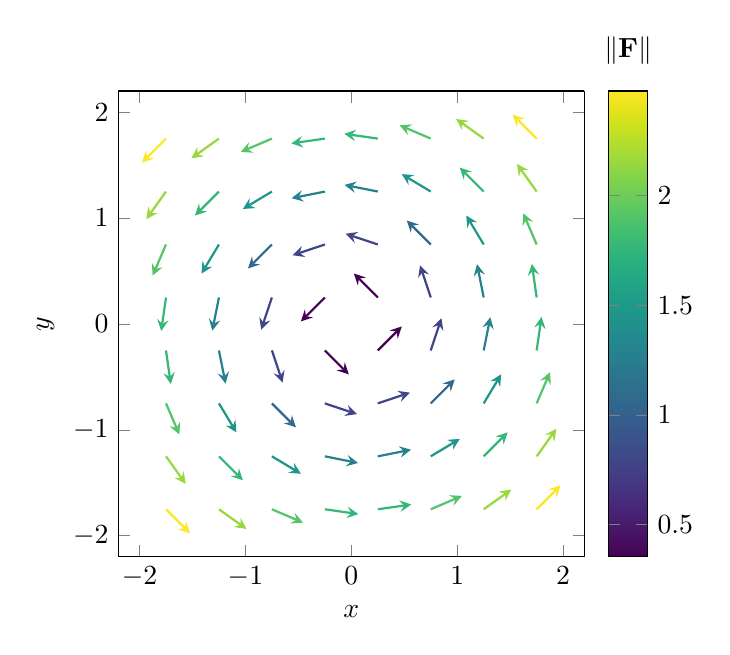
\begin{tikzpicture}
  \begin{axis}[
    width=7.5cm, height=7.5cm, view={0}{90}, axis equal image,
    xmin=-2.2, xmax=2.2, ymin=-2.2, ymax=2.2, zmin=-1, zmax=1,
    xlabel=$x$, ylabel=$y$, colormap/viridis, colorbar,
    colorbar style={title={$\|\mathbf{F}\|$}},
  ]
    \addplot3[point meta={sqrt(x^2 + y^2)}, -stealth, thick,
      quiver={u={-y/sqrt(x^2 + y^2)}, v={x/sqrt(x^2 + y^2)}, scale arrows=0.32, colored},
      domain=-1.75:1.75, domain y=-1.75:1.75, samples=8] {0};
  \end{axis}
\end{tikzpicture}
